% AstroAgentBench — AACL-IJCNLP 2026 poster (A0 portrait)
% Build: latexmk -pdf -interaction=nonstopmode -halt-on-error -outdir=build poster.tex
\documentclass[final]{beamer}

\usepackage[orientation=portrait,size=a0,scale=1.0]{beamerposter}
\usetheme{default}
\usepackage[T1]{fontenc}
\usepackage[utf8]{inputenc}
\usepackage{helvet}
\renewcommand{\familydefault}{\sfdefault}
\usepackage{graphicx}
\usepackage{booktabs}
\usepackage{colortbl}
\usepackage{tabularx}

\definecolor{abnavy}{HTML}{102C51}
\definecolor{abcyan}{HTML}{0096BF}
\definecolor{ablight}{HTML}{EAF3F8}
\definecolor{abgray}{HTML}{5A6B7C}
\definecolor{abgold}{HTML}{B8862D}
\definecolor{abred}{HTML}{B03A2E}

\setbeamercolor{normal text}{fg=abnavy,bg=white}
\setbeamercolor{structure}{fg=abcyan}
\setbeamercolor{block title}{bg=abnavy,fg=white}
\setbeamercolor{block body}{bg=white,fg=abnavy}
\setbeamercolor{headline}{bg=abnavy,fg=white}
\setbeamercolor{resourcestrip}{bg=ablight,fg=abnavy}
\setbeamercolor{workedbox}{bg=ablight,fg=abnavy}
\setbeamercolor{takeaway}{bg=abnavy,fg=white}
\setbeamercolor{footline}{bg=ablight,fg=abnavy}

\setbeamertemplate{navigation symbols}{}
\setbeamertemplate{itemize item}{\textcolor{abcyan}{\raisebox{0.12em}{\scriptsize$\blacksquare$}}}
\setbeamertemplate{itemize subitem}{\textcolor{abcyan}{--}}

\setbeamertemplate{block begin}{%
  \vskip 1.6ex
  \begin{beamercolorbox}[rounded=true,sep=0.5em,leftskip=0.8em]{block title}%
    {\Large\bfseries\insertblocktitle\par}%
  \end{beamercolorbox}%
  \begin{beamercolorbox}[rounded=true,sep=0.9em]{block body}%
}
\setbeamertemplate{block end}{%
  \end{beamercolorbox}\vskip 1.8ex
}

\newcommand{\bnum}[1]{\textcolor{abcyan}{\bfseries #1}\;\;}
\newcommand{\stat}[2]{{\centering{\Huge\bfseries\color{abcyan}#1\par}\vspace{0.1em}{\normalsize\color{abgray}#2\par}}}
\newcommand{\srcnote}[1]{{\small\color{abgray}#1\par}}

\graphicspath{{../assets/}}

\begin{document}

\begin{frame}[t,fragile]

% ==================== Headline ====================
\begin{beamercolorbox}[wd=\paperwidth,sep=1.0em]{headline}
  \begin{columns}[T]
    \column{0.11\paperwidth}
      \vspace{0.7em}\hspace{1.2em}
\includegraphics[width=0.86\linewidth]{logo-dark.pdf}
    \column{0.71\paperwidth}
      \vspace{0.1em}
      {\veryHuge\bfseries AstroAgentBench: Evaluating Agentic Planning on Space Mission Planning Tasks\par}
      \vspace{0.3em}
      {\Large\bfseries\color{abcyan} A valid plan can still accomplish little.\par}
      \vspace{0.35em}
      {\Large Weiyi Wang\textsuperscript{1,5}\quad Xinchi Chen\textsuperscript{1,3,4,5}\,\textsuperscript{\dag}\quad Jingjing Gong\textsuperscript{2,5}\quad Xuanjing Huang\textsuperscript{1,4}\quad Xipeng Qiu\textsuperscript{1,2,3,4,5}\,\textsuperscript{\dag}\par}
      \vspace{0.25em}
      {\normalsize\color{ablight}
      \textsuperscript{1}\,Institute of Trustworthy Embodied AI, Fudan University \,\textperiodcentered\,
      \textsuperscript{2}\,Shanghai Innovation Institute \,\textperiodcentered\,
      \textsuperscript{3}\,Shanghai Key Laboratory of Multimodal Embodied AI \,\textperiodcentered\,
      \textsuperscript{4}\,College of Computer Science and Artificial Intelligence, Fudan University \,\textperiodcentered\,
      \textsuperscript{5}\,OpenMOSS Team\par}
    \column{0.18\paperwidth}
      \vspace{0.7em}\centering
      {\LARGE\bfseries\color{abcyan} AACL-IJCNLP 2026\par}
      \vspace{0.4em}
      {\footnotesize\color{ablight} All resources are one scan away.\par}
  \end{columns}
\end{beamercolorbox}

% ==================== Resource strip ====================
\begin{beamercolorbox}[wd=\paperwidth,sep=0.5em]{resourcestrip}
  \centering
  \begin{columns}[T]
    \column{0.23\paperwidth}\centering
      
\includegraphics[width=0.055\paperwidth]{qr_github.png}\par\vspace{0.15em}
      {\small\bfseries Code \& cases}\par {\scriptsize github.com/\\Mtrya/AstroAgentBench}
    \column{0.23\paperwidth}\centering
      
\includegraphics[width=0.055\paperwidth]{qr_hf.png}\par\vspace{0.15em}
      {\small\bfseries Taskset}\par {\scriptsize Hugging Face}
    \column{0.23\paperwidth}\centering
      
\includegraphics[width=0.055\paperwidth]{qr_arxiv.png}\par\vspace{0.15em}
      {\small\bfseries Paper}\par {\scriptsize arXiv 2601.11354}
    \column{0.23\paperwidth}\centering
      
\includegraphics[width=0.055\paperwidth]{qr_zenodo.png}\par\vspace{0.15em}
      {\small\bfseries Run archive}\par {\scriptsize Zenodo}
  \end{columns}
\end{beamercolorbox}

\vspace{1.0em}

% ==================== Body: 3 columns ====================
\begin{columns}[t]

% -------------------- Column 1 --------------------
\column{0.315\paperwidth}

\begin{block}{\bnum{1}Space mission planning: consequential, difficult, executable}
  \centering
  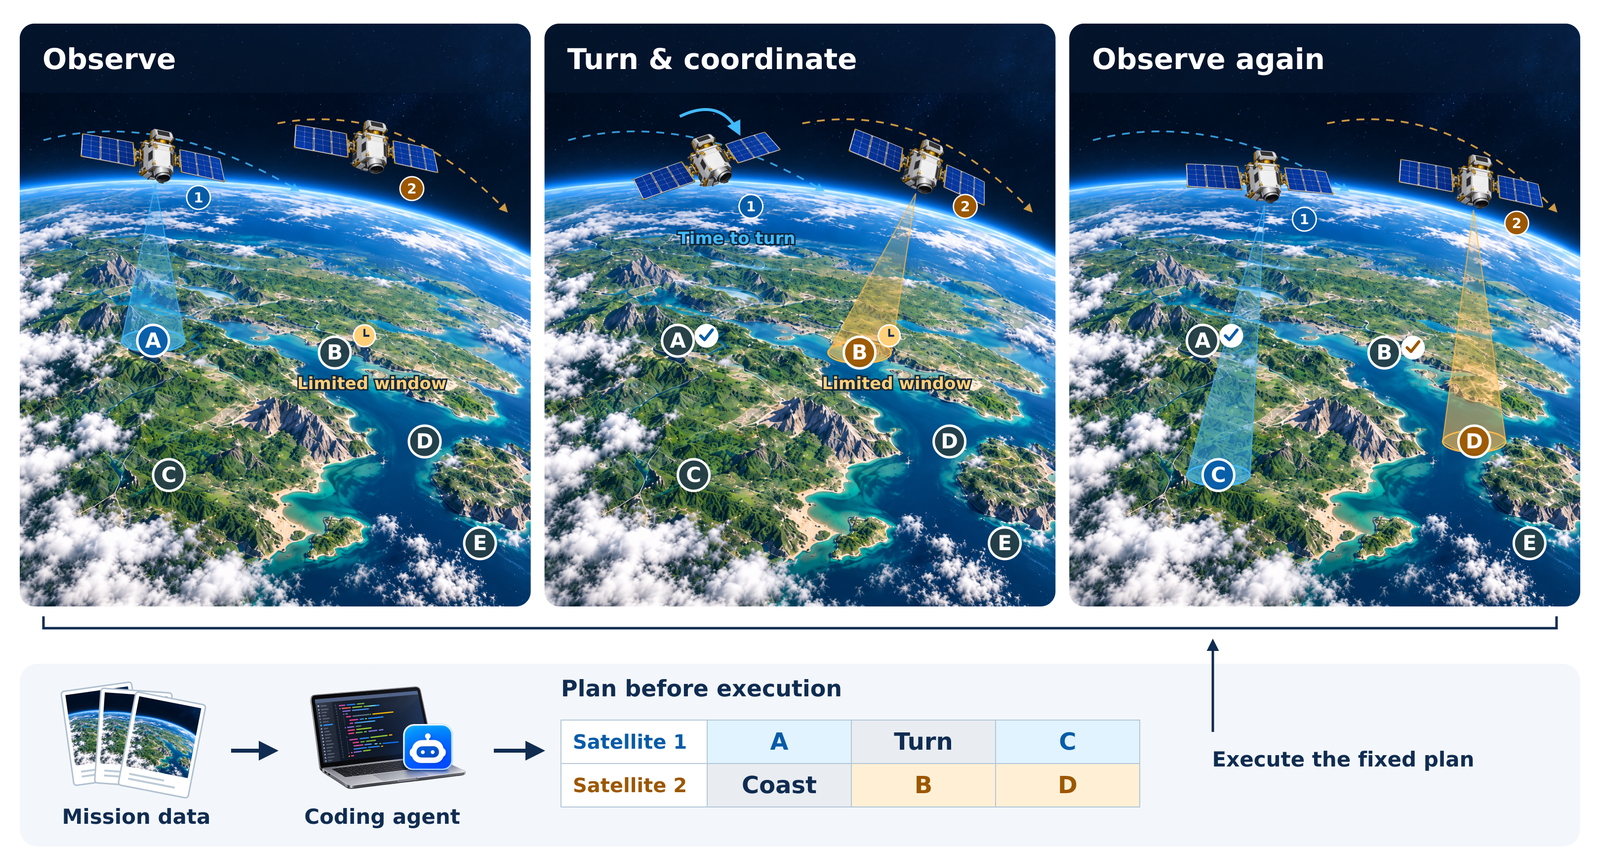
\includegraphics[width=0.80\linewidth]{mission-planning-crop.png}
  \par\vspace{0.7em}
  \raggedright
  Mission goals translate into executable decisions over spacecraft, ground assets, crosslinks, energy, data storage, and timing. These elements are tightly coupled over extended operational horizons and constrained by physics. A plan that appears plausible in natural language can still violate visibility, slewing, or power constraints; crucially, the plan is committed \textbf{before execution}.
  \par\vspace{0.5em}
  {\color{abcyan}\bfseries Can an LLM agent compute a mission plan that survives contact with a physical simulation model?}
  \par\vspace{0.3em}
  \srcnote{Illustrative Earth-observation mission; geometry and timing are schematic.}
\end{block}

\begin{block}{\bnum{2}The evaluation gap}
  \begin{itemize}\setlength{\itemsep}{0.25em}
    \item LLM-for-Space systems are evaluated under \textbf{different task contracts, simulators, and success criteria}.
    \item Validity alone is too weak: a plan can satisfy a schema and still \textbf{observe nothing of value}.
    \item What is missing: \textbf{physically grounded planning verifiable against a domain model}.
  \end{itemize}
  \vspace{0.4em}
  \textbf{Three questions:} \textbf{Q1} Can agents pass external feasibility checks? \textbf{Q2} When valid, how closely does plan quality approach specialized solver references? \textbf{Q3} Which system conditions (verifier usage, procedural guidance, memory) explain performance variation?
\end{block}

\begin{block}{\bnum{3}Benchmark: case in, executable plan out, verifier decides}
  \centering
  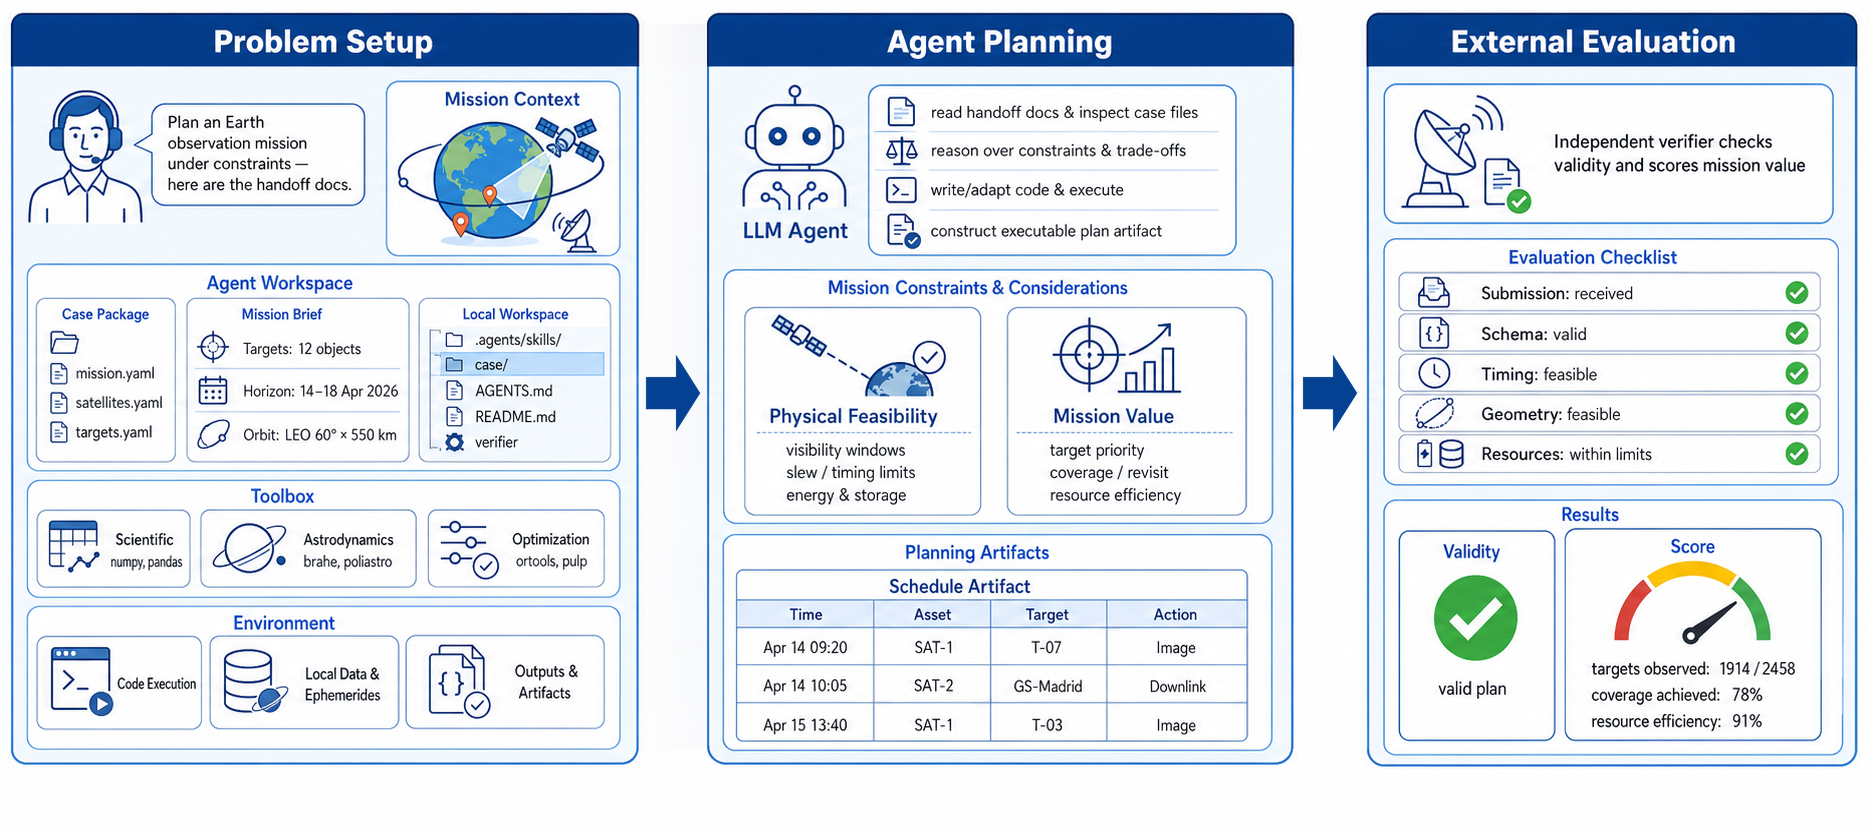
\includegraphics[width=0.86\linewidth]{overview.png}
  \par\vspace{0.7em}
  \raggedright
  Each case packages mission parameters, an engineering brief, libraries, a solution schema, and a local verifier utility. The agent \textbf{synthesizes the planning procedure autonomously} (no pre-built domain planner is provided). An independent external verifier re-simulates physics to validate constraints and score mission value.
\end{block}

\begin{block}{\bnum{4}Seven families, four kinds of planning decisions}
  \begin{columns}[t]
    \column{0.24\linewidth}\centering
      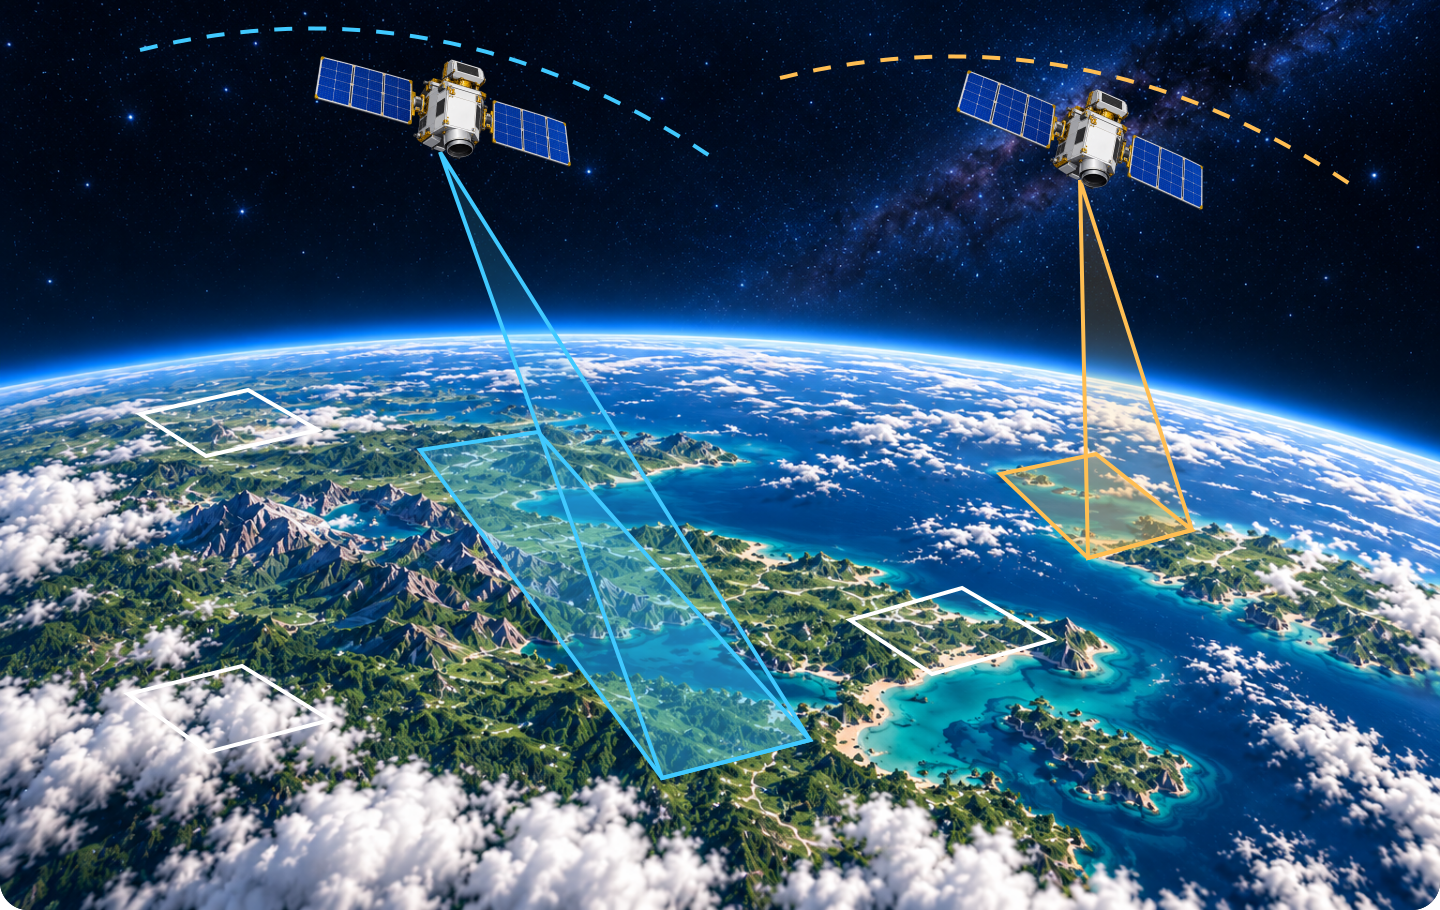
\includegraphics[width=0.78\linewidth]{tour-observe.png}\par\vspace{0.2em}
      {\footnotesize\bfseries Observe Earth}\par {\scriptsize AEOSSP \,\textperiodcentered\, SPOT-5\\ Regional \,\textperiodcentered\, Stereo}
    \column{0.24\linewidth}\centering
      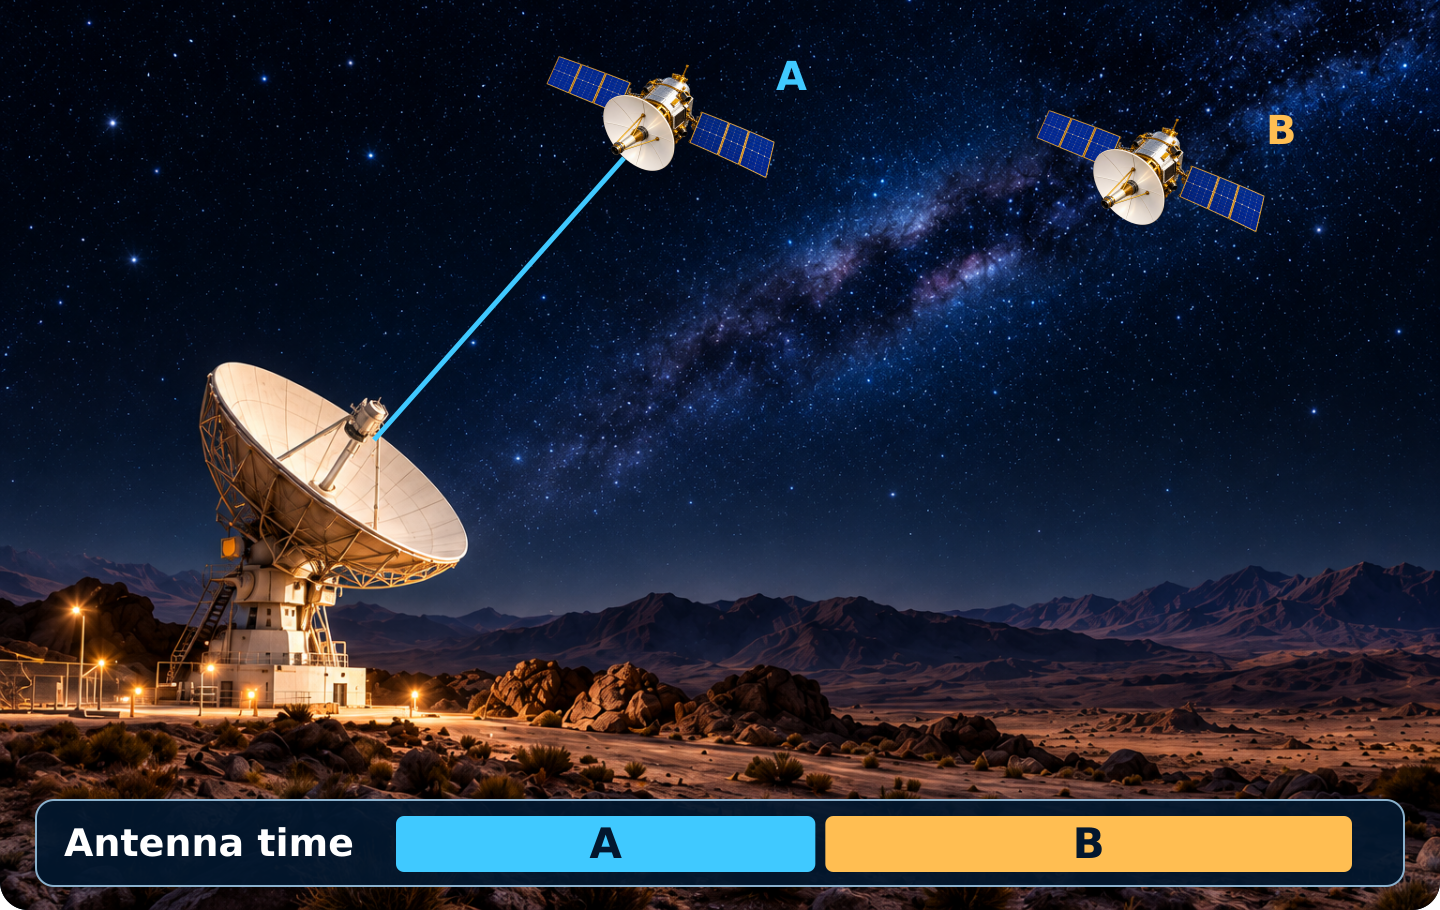
\includegraphics[width=0.78\linewidth]{tour-contacts.png}\par\vspace{0.2em}
      {\footnotesize\bfseries Allocate contacts}\par {\scriptsize SatNet}
    \column{0.24\linewidth}\centering
      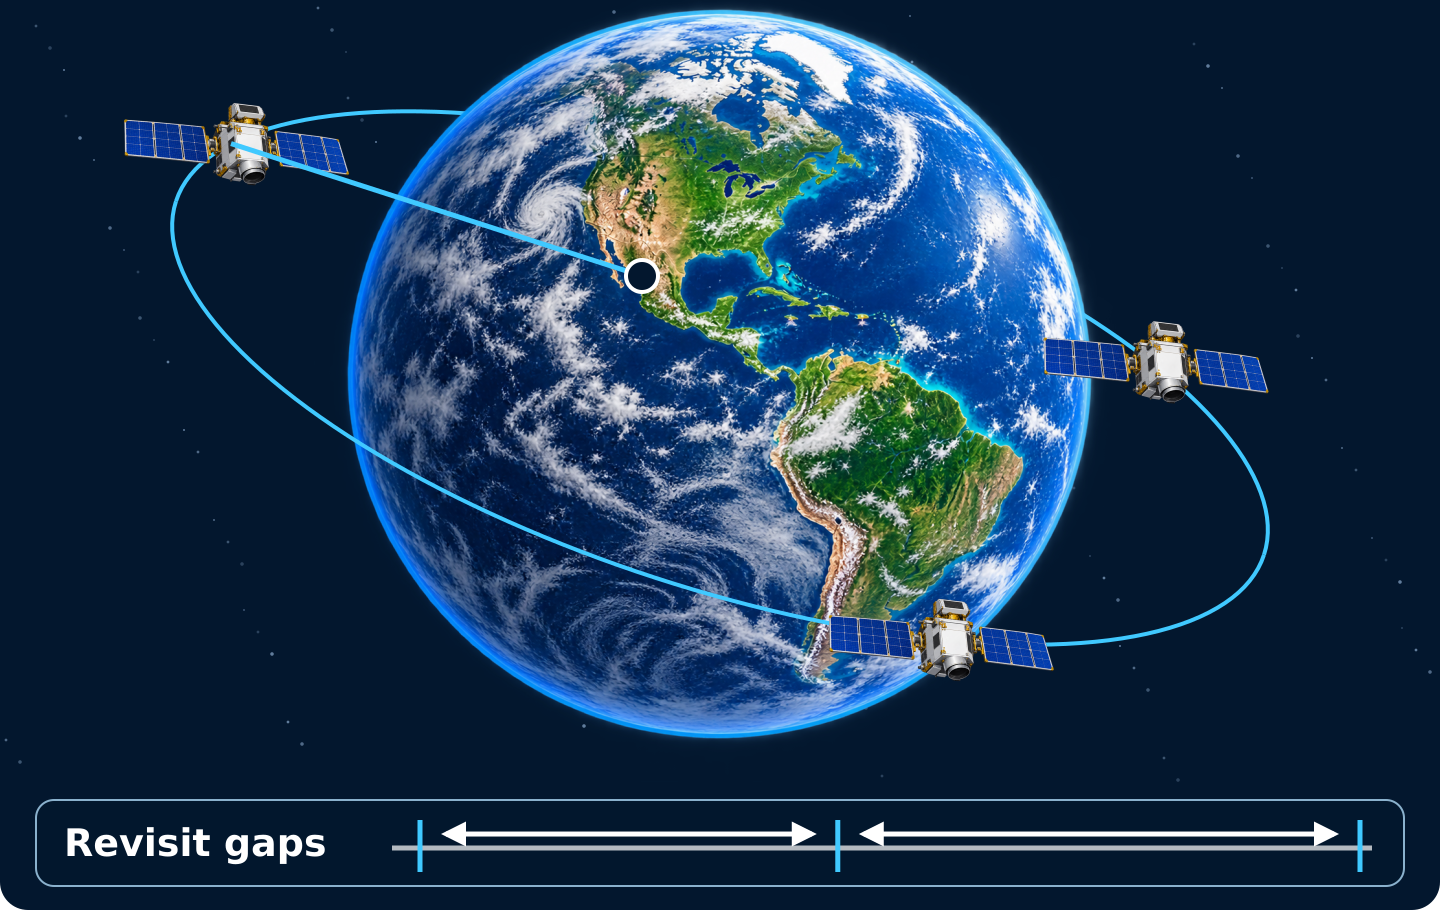
\includegraphics[width=0.78\linewidth]{tour-revisit.png}\par\vspace{0.2em}
      {\footnotesize\bfseries Design constellations}\par {\scriptsize Revisit}
    \column{0.24\linewidth}\centering
      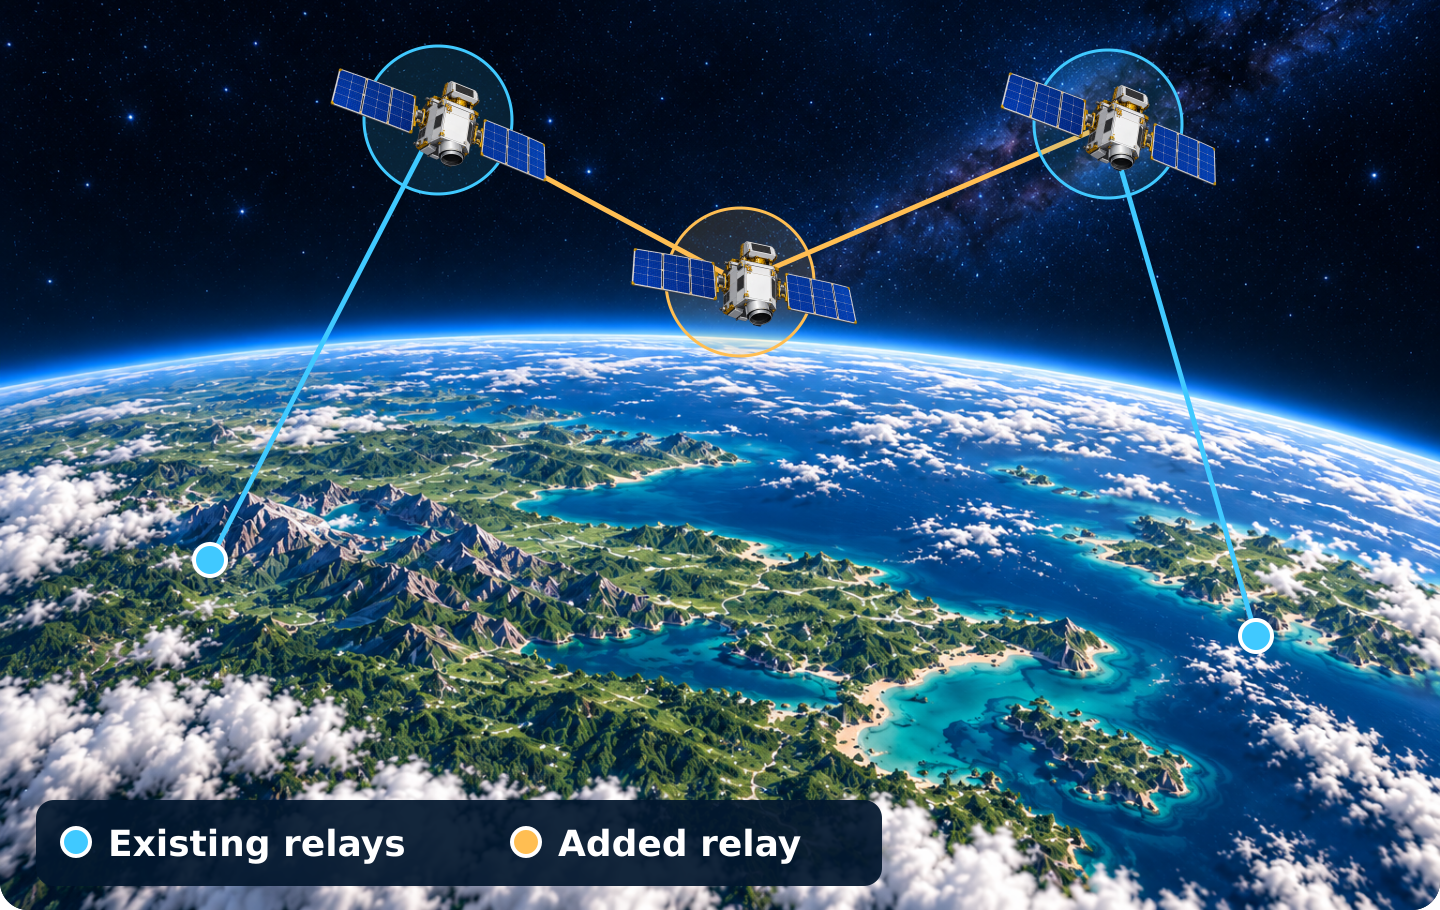
\includegraphics[width=0.78\linewidth]{tour-relay.png}\par\vspace{0.2em}
      {\footnotesize\bfseries Augment relay networks}\par {\scriptsize Relay}
  \end{columns}
  \vspace{0.4em}
  {\footnotesize
  \setlength{\tabcolsep}{4pt}
  \begin{tabularx}{\linewidth}{@{}l X r@{}}
    \toprule
    \textbf{Decision} & \textbf{The agent submits} & \textbf{Per-case scale} \\
    \midrule
    Observe Earth & schedule, photograph, strip, stereo pair & 8 photos--18.3k cells \\
    Allocate contacts & antenna-track assignment & 257--333 requests; 7\,d \\
    Design constellations & constellation states + schedule & 24--32 targets; 48\,h \\
    Augment relay networks & added satellites + link plan & 6--10 sats; 4--8 demands \\
    \bottomrule
  \end{tabularx}}
  \par\vspace{0.4em}
  \srcnote{116 cases (60 train / 35 held-out test / auxiliary). Orbits from real CelesTrak TLE snapshots; targets from public city/site/region libraries; SatNet \& SPOT-5 normalized from published benchmarks.}
\end{block}

% -------------------- Column 2 --------------------
\column{0.315\paperwidth}

\begin{block}{\bnum{5}Validity first, then mission value}
  \textbf{Validity} (strict physical constraints re-simulated by the verifier):
  \begin{itemize}\setlength{\itemsep}{0.1em}
    \item Submission \,\textperiodcentered\, Schema: artifact exists and parses cleanly
    \item Time \,\textperiodcentered\, Geometry \,\textperiodcentered\, Resources: visibility windows, pointing angles, concurrent tasks, battery margins, onboard memory
  \end{itemize}
  \vspace{0.4em}
  \textbf{Performance} (evaluated only if valid): family-native value (task completion, geographic coverage, contact duration, revisit gap, profit) mapped to a normalized 0--100 scale; missing or invalid submissions score zero.
  \par\vspace{0.5em}
  {\small \textbf{AEOSSP case 1:} 70.87 (1,415/1,947 tasks; 68.5\% of task weight); five-case mean 58.45. The two measurements are decoupled.}
\end{block}

\begin{block}{\bnum{6}Main results: agents plan for real, yet performance varies widely}
  \centering
  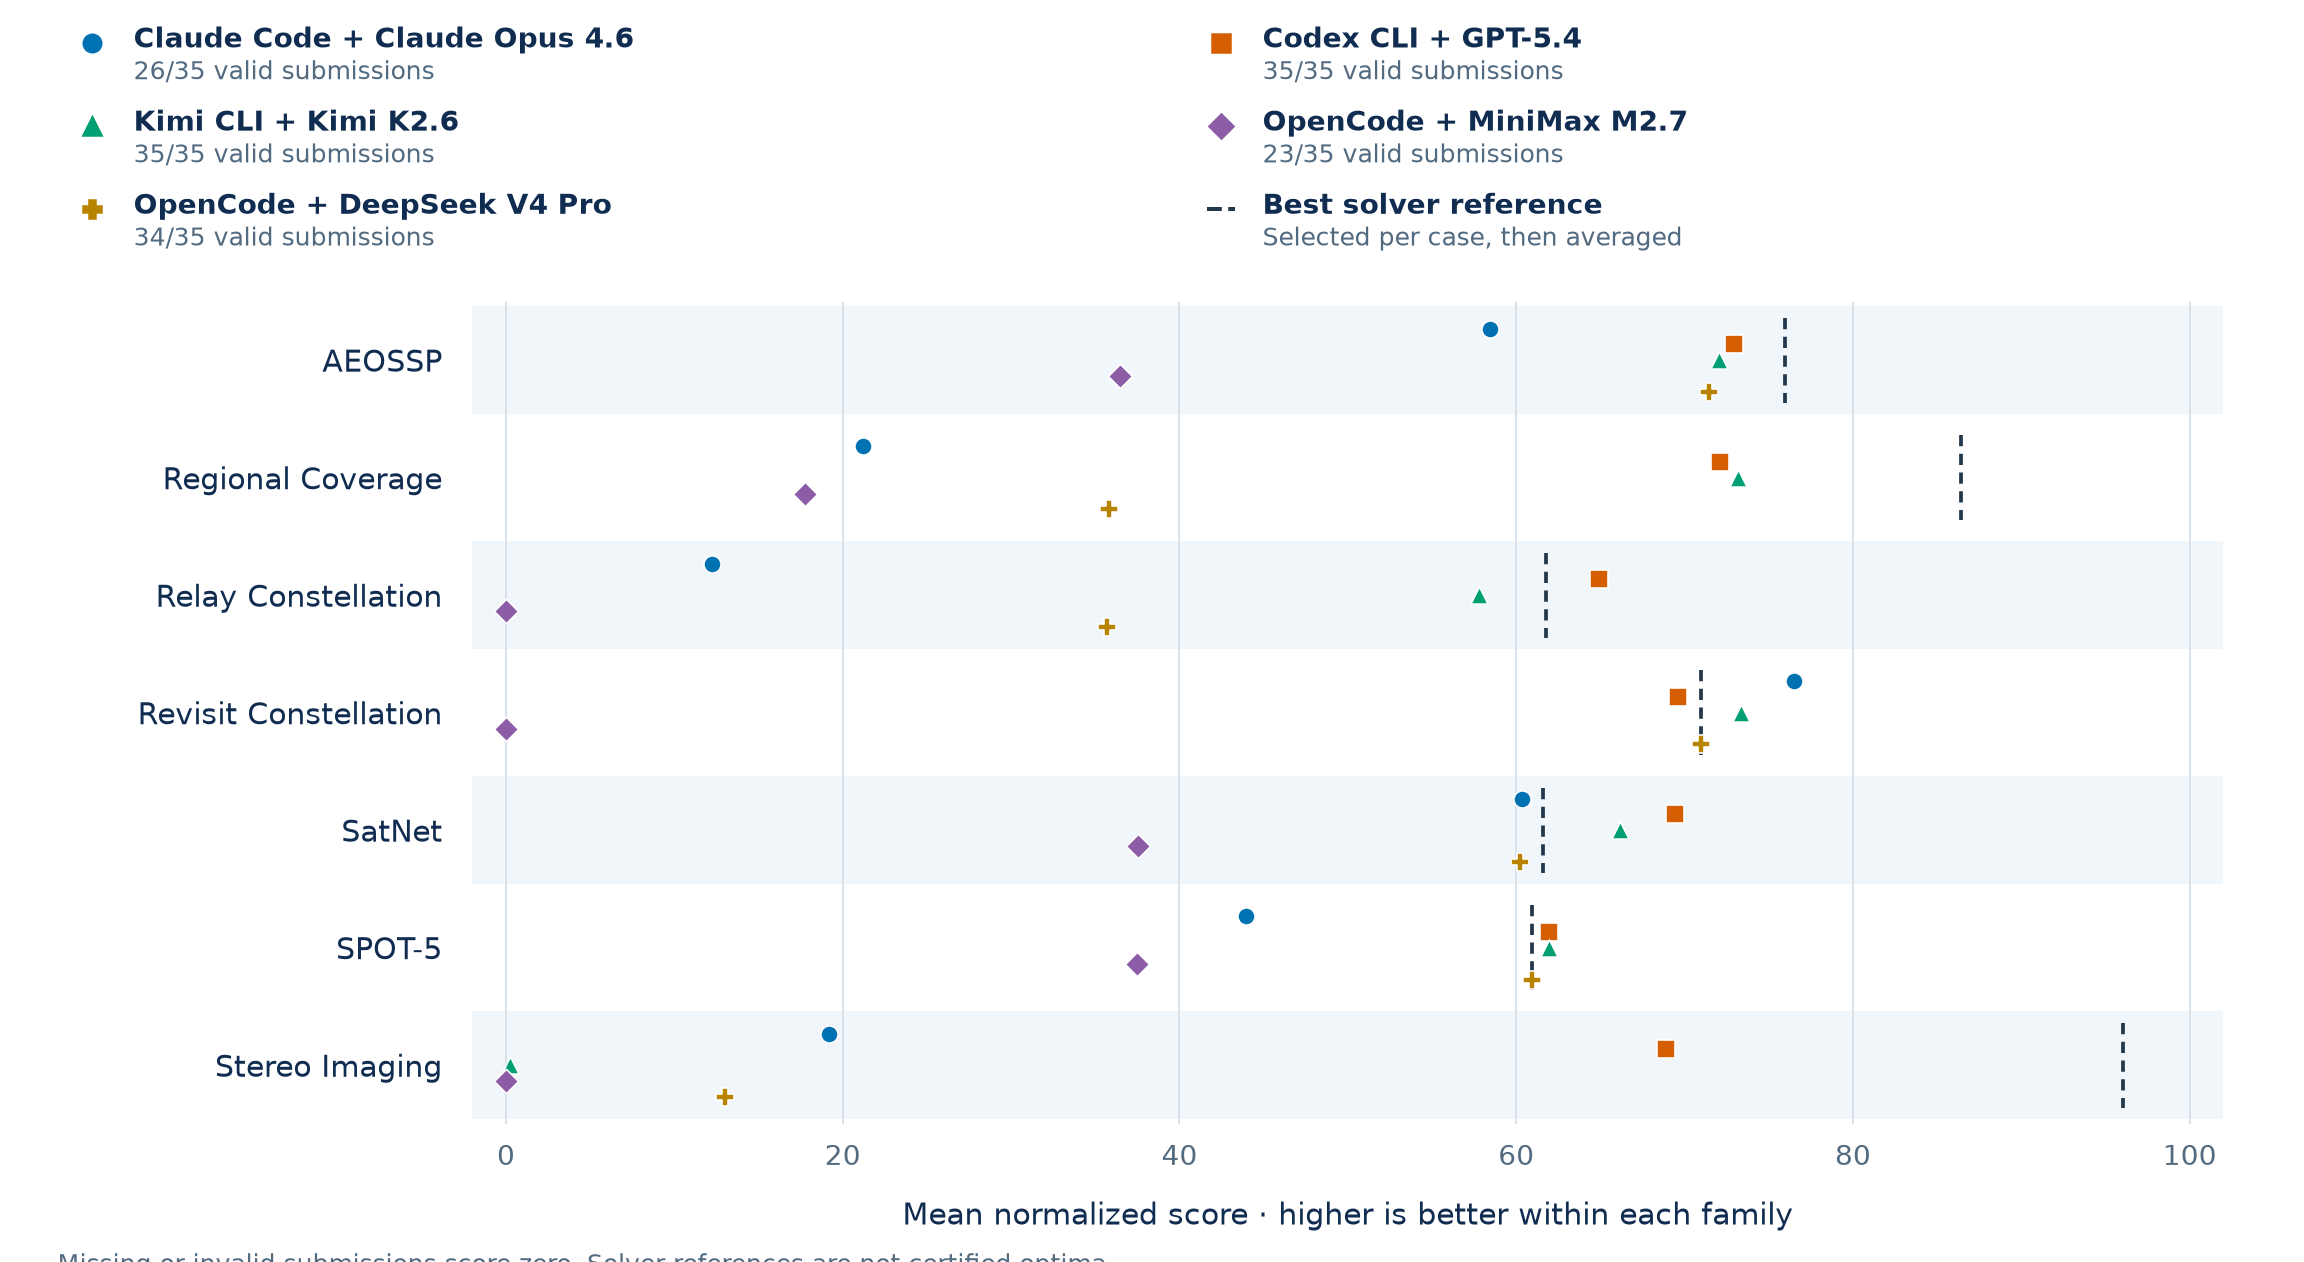
\includegraphics[width=0.96\linewidth]{initial-results-plot.png}
  \par\vspace{0.7em}
  \begin{columns}[t]
    \column{0.32\linewidth}\stat{35/35}{verifier-valid submissions (Codex + GPT-5.4; Kimi + K2.6), yet valid $\neq$ valuable}
    \column{0.32\linewidth}\stat{4 / 7}{families where the top agent row outperforms solver baselines (SPOT-5, Relay, Revisit, SatNet)}
    \column{0.32\linewidth}\stat{13–27}{point gaps remain on Regional Coverage and Stereo Imaging}
  \end{columns}
  \vspace{0.5em}
  \raggedright
  {\small \textbf{Setup.} Five systems (Claude Code/Opus 4.6; Codex/GPT-5.4; Kimi/K2.6; OpenCode with MiniMax M2.7 and DeepSeek V4 Pro), 35 held-out cases, 2\,h on 8 cores, scored post-run without human repair. Capability is uneven: family leaders differ across systems.}
\end{block}

\begin{block}{\bnum{7}Where runs fail: two distinct layers}
  \textbf{1. Task-formulation failures.} The system builds a \textbf{self-imposed task} from rich files: inferred schema, hallucinated objective. \emph{Stereo Imaging:} valid observations whose footprints never form stereo products; local validation accepts what the official verifier rejects.
  \par\vspace{0.4em}
  \textbf{2. Solution-construction failures.} The task is understood, but the run cannot \textbf{build, improve, and preserve} a high-value plan (weak search, brittle code, late verifier use). \emph{Relay:} valid-but-zero-value submissions accepted as done.
  \par\vspace{0.6em}
  \begin{columns}[t]
    \column{0.32\linewidth}\stat{\textcolor{abred}{12.6\%}}{of 175 runs invalid}
    \column{0.32\linewidth}\stat{\textcolor{abred}{9.1\%}}{valid yet zero score}
    \column{0.32\linewidth}\stat{\textcolor{abred}{22.3\%}}{artifact before contract}
  \end{columns}
\end{block}

% -------------------- Column 3 --------------------
\column{0.315\paperwidth}

\begin{block}{\bnum{8}Three traces, three mechanisms}
  \centering
  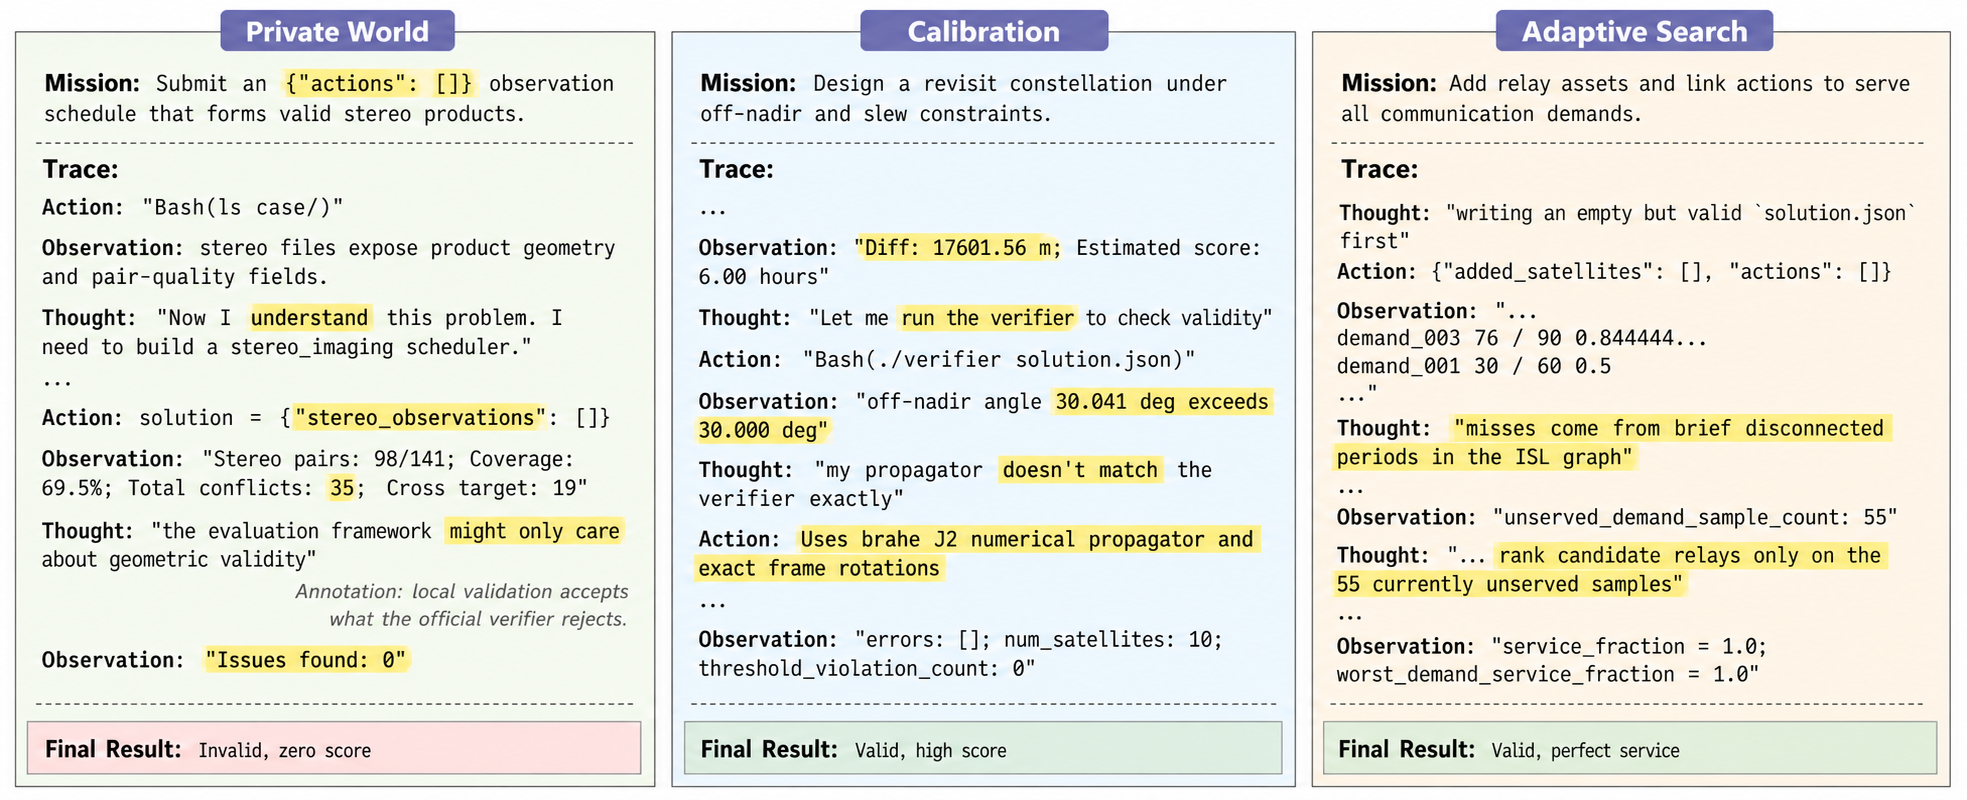
\includegraphics[width=0.99\linewidth]{case_study.png}
  \par\vspace{0.6em}
  \raggedright
  \textbf{Left:} a self-imposed task contract fails the official check. \textbf{Middle:} verifier disagreement repairs the agent-written orbital model. \textbf{Right:} search targets the 55 unserved demands; the valid incumbent is preserved.
\end{block}

\begin{block}{\bnum{9}What strong runs do differently}
  \begin{itemize}\setlength{\itemsep}{0.35em}
    \item \textbf{Implementation calibration}: agent-written propagation, geometry, and scheduling code is systematically repaired against \textbf{verifier disagreement} before being trusted.
    \item \textbf{Case-adaptive search with incumbent preservation}: the run identifies the specific bottleneck of the target instance (bridge relays, unserved demands, or satellite counts) and continuously safeguards its best verified plan.
  \end{itemize}
  \vspace{0.3em}
  Solvers are systematic but operate under fixed policies; high-performing agent runs \textbf{synthesize and adapt search strategies dynamically during execution}.
\end{block}

\begin{block}{\bnum{10}Workspace support aids planning conditionally}
  \begin{columns}[t]
    \column{0.49\linewidth}\centering
      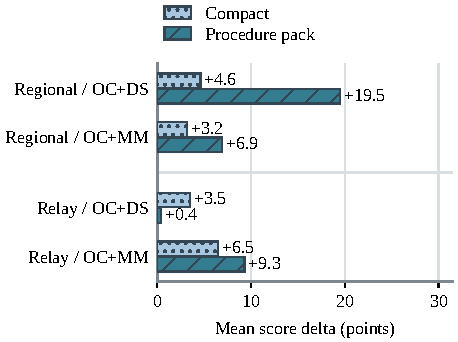
\includegraphics[width=0.94\linewidth]{ablation_procedure.pdf}\par\vspace{0.2em}
      {\normalsize\bfseries (A) Procedure injection}
    \column{0.49\linewidth}\centering
      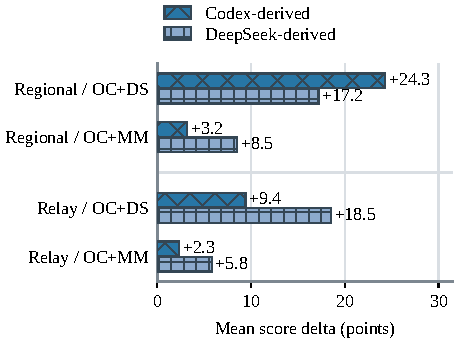
\includegraphics[width=0.94\linewidth]{ablation_memory.pdf}\par\vspace{0.2em}
      {\normalsize\bfseries (B) Memory accumulation}
  \end{columns}
  \vspace{0.3em}
  Score deltas vs.\ no-support baseline (OpenCode systems; Regional \& Relay). Support helps \textbf{when it supplies the missing formulation, calibration, or search discipline}.
\end{block}

\begin{beamercolorbox}[rounded=true,sep=1.0em,wd=\linewidth]{takeaway}
  {\Large\bfseries Take-home message\par}
  \vspace{0.5em}
  {\LARGE\bfseries A valid plan can still accomplish little.\par}
  \vspace{0.5em}
  {\normalsize Success tracks \textbf{verifier-calibrated implementations} and \textbf{disciplined, case-adaptive search}: an agent-\emph{system} property, not a model-only attribute.\par}
  \vspace{0.4em}
  {\small Code, cases, verifiers, solver references, and run traces are public.\par}
\end{beamercolorbox}

\end{columns}

\end{frame}
\end{document}
